   \begin{figure}[!htb]
      \centering
      \setlength{\abovecaptionskip}{6pt plus 1pt minus 1pt}
      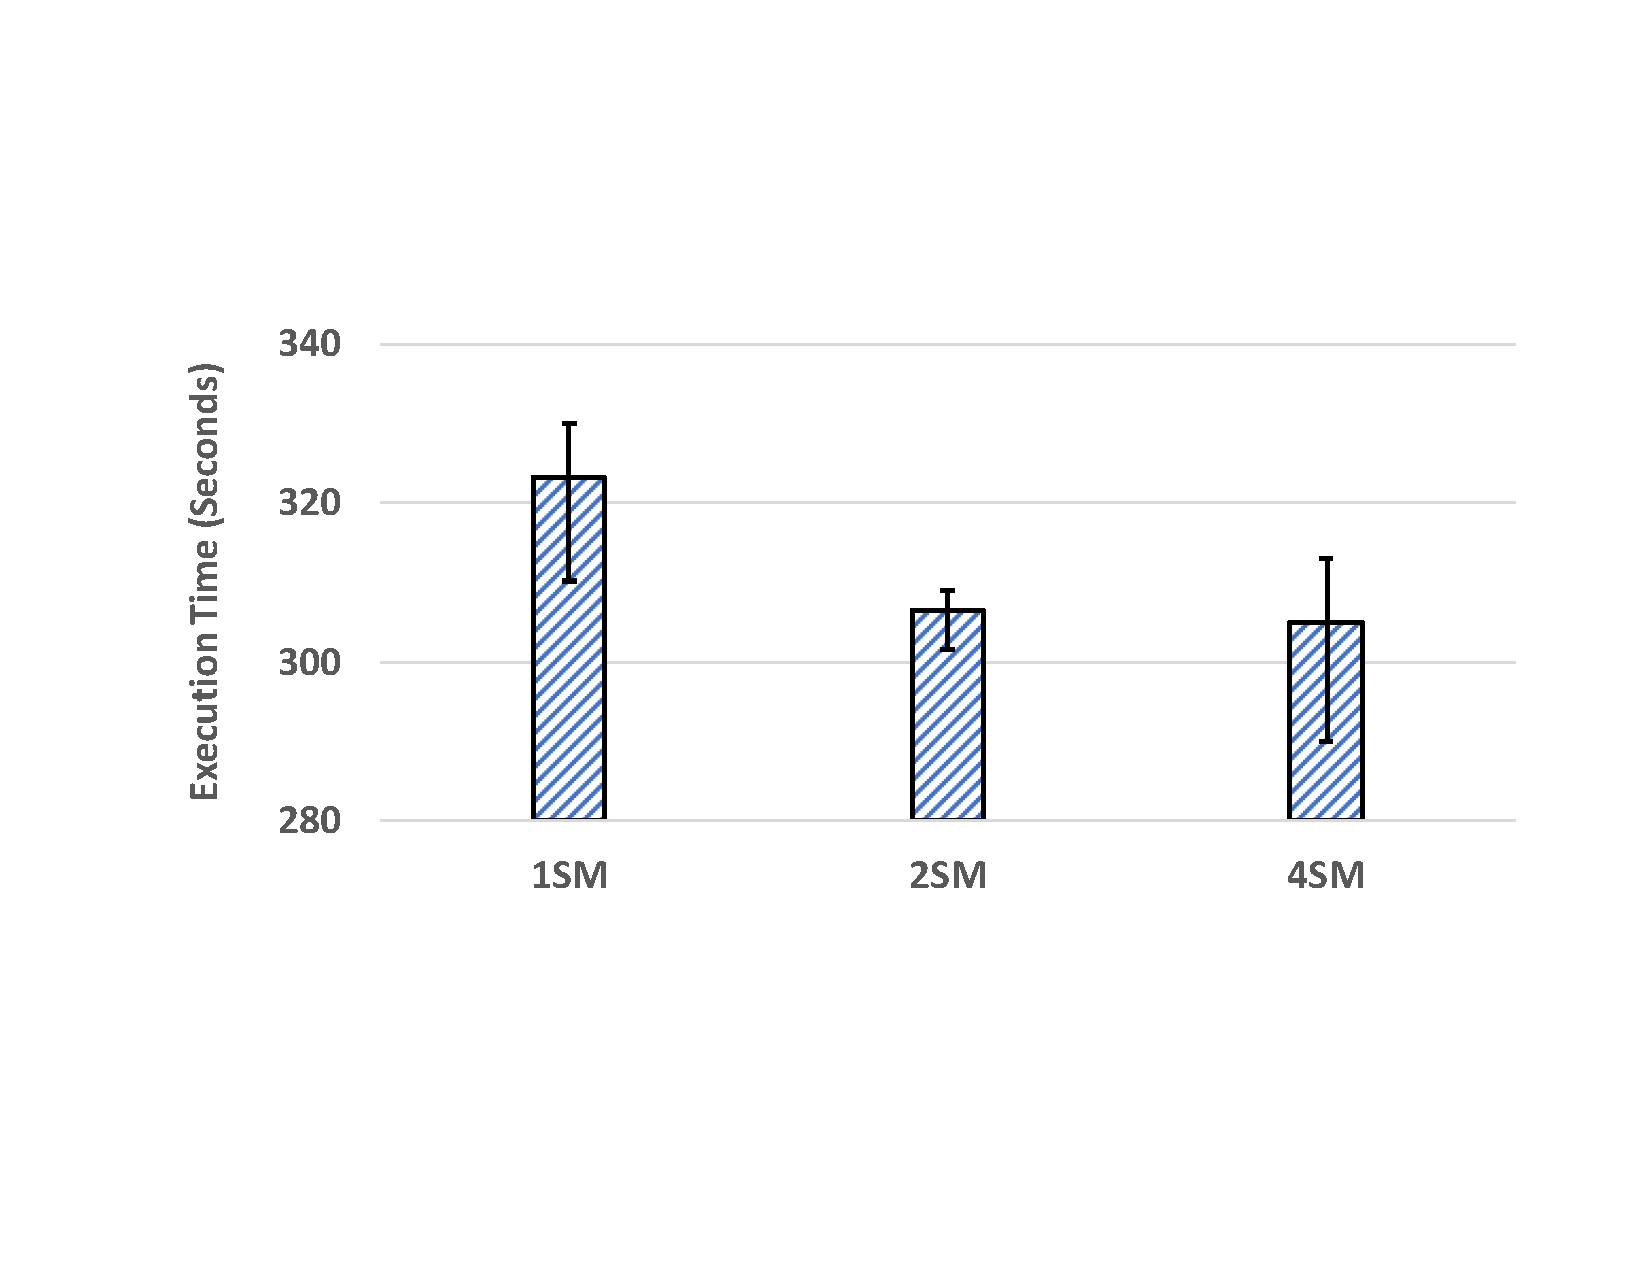
\includegraphics[width=.90\textwidth,keepaspectratio]{figures/par-perf.pdf}
      \captionsetup{width=.90\textwidth}
      \caption{SST-GPU total executon time with the different numbers of SM groups for V100 Volta GPU.
       We run 5 times for each configuration and mark the average as well as the maximum and minimum
       execution time in this figure.}
      \label{fig:par-perf}
   \end{figure}

To show the parallel simulation performance with SST-GPU, we split V100 Volta GPU
into 1, 2, and 4 SM groups and put each SM group in one thread. To show the advantage
of parallel simulation, we use Vector Addition application and accumulate input vector elements
2000 times to its output vector elements. Thus, each thread cause more time at computing
but not memory accesses. We launch 84 CTAs and each with 256 threads to make sure at least
1 CTA per SM.

Figure \ref{fig:par-perf} shows the total time cost to run Vector Addition
with the different numbers of SM groups. We assign CPU and its memory to one thread and
each of the SM group and its memory hierarchy to one thread. The GPU scheduler is attached
to the first SM group thread. We achieve on average 5\% speedup with 2 SM groups. Note that
a significant amount of time are due to initialization, configuration, and memory copy.
